\documentclass[12pt]{article}
\usepackage{amsfonts, amssymb, amsmath, amsthm}
\usepackage[margin=1in]{geometry}
\usepackage{tikz}
\usetikzlibrary{patterns, decorations.pathreplacing}

\pagestyle{myheadings}
\markright{Explainer: Rudin 4.8 --- Uniform Continuity and Boundedness\hfill}

\newcommand{\R}{\mathbb{R}}
\newcommand{\eps}{\varepsilon}

\begin{document}

\begin{center}
    \textbf{\Large Uniform Continuity and Boundedness}\\[0.5em]
    \large A visual guide to Rudin 4.8
\end{center}

\section{Uniform Continuity vs Regular Continuity}

\begin{center}
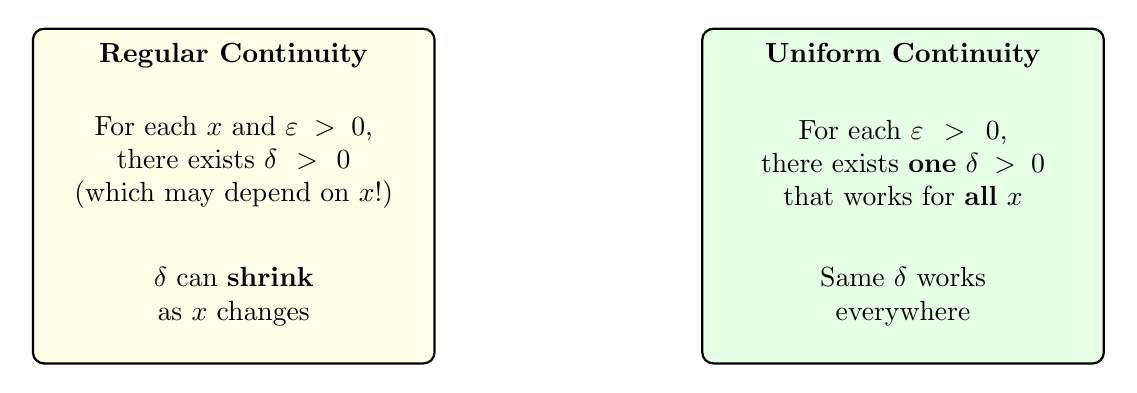
\begin{tikzpicture}[scale=0.85]
    % Regular continuity
    \begin{scope}[xshift=-5cm]
        \draw[thick, rounded corners, fill=yellow!10] (-3, -2.5) rectangle (3, 2.5);
        \node at (0, 2.1) {\textbf{Regular Continuity}};

        \node[text width=5cm, align=center] at (0, 0.5) {For each $x$ and $\eps > 0$,\\there exists $\delta > 0$\\(which may depend on $x$!)};

        \node[text width=5cm, align=center] at (0, -1.5) {$\delta$ can \textbf{shrink}\\as $x$ changes};
    \end{scope}

    % Uniform continuity
    \begin{scope}[xshift=5cm]
        \draw[thick, rounded corners, fill=green!10] (-3, -2.5) rectangle (3, 2.5);
        \node at (0, 2.1) {\textbf{Uniform Continuity}};

        \node[text width=5cm, align=center] at (0, 0.5) {For each $\eps > 0$,\\there exists \textbf{one} $\delta > 0$\\that works for \textbf{all} $x$};

        \node[text width=5cm, align=center] at (0, -1.5) {Same $\delta$ works\\everywhere};
    \end{scope}
\end{tikzpicture}
\end{center}

\section{The Claim}

\begin{center}
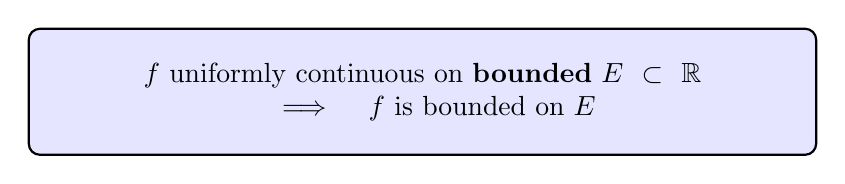
\begin{tikzpicture}
    \draw[thick, rounded corners, fill=blue!10] (-5, -0.8) rectangle (5, 0.8);
    \node[text width=9cm, align=center] at (0, 0) {
        $f$ uniformly continuous on \textbf{bounded} $E \subset \R$\\
        $\implies$ $f$ is bounded on $E$
    };
\end{tikzpicture}
\end{center}

\section{The Chaining Argument}

Since $E$ is bounded, it fits inside some interval $[a, b]$. The key idea: walk across $E$ in steps of size $\delta$, and $f$ can only change by $\eps$ each step.

\begin{center}
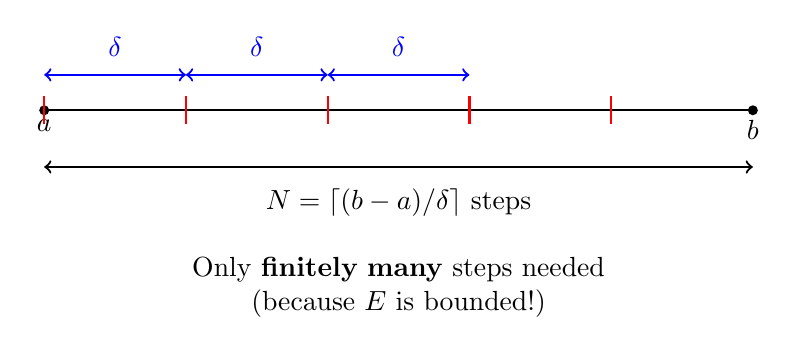
\begin{tikzpicture}[scale=0.9]
    % The interval
    \draw[thick] (0, 0) -- (10, 0);
    \fill (0, 0) circle (2pt) node[below] {$a$};
    \fill (10, 0) circle (2pt) node[below] {$b$};

    % Delta steps
    \foreach \i in {0, 1, 2, 3, 4} {
        \pgfmathsetmacro{\x}{2*\i}
        \draw[red, thick] (\x, -0.2) -- (\x, 0.2);
    }

    % Delta brackets
    \draw[<->, blue, thick] (0, 0.5) -- (2, 0.5);
    \node[blue] at (1, 0.9) {$\delta$};
    \draw[<->, blue, thick] (2, 0.5) -- (4, 0.5);
    \node[blue] at (3, 0.9) {$\delta$};
    \draw[<->, blue, thick] (4, 0.5) -- (6, 0.5);
    \node[blue] at (5, 0.9) {$\delta$};

    % Number of steps
    \draw[<->, thick] (0, -0.8) -- (10, -0.8);
    \node at (5, -1.3) {$N = \lceil(b-a)/\delta\rceil$ steps};

    \node[text width=9cm, align=center] at (5, -2.5) {Only \textbf{finitely many} steps needed\\(because $E$ is bounded!)};
\end{tikzpicture}
\end{center}

\subsection{How the Bound Works}

\begin{center}
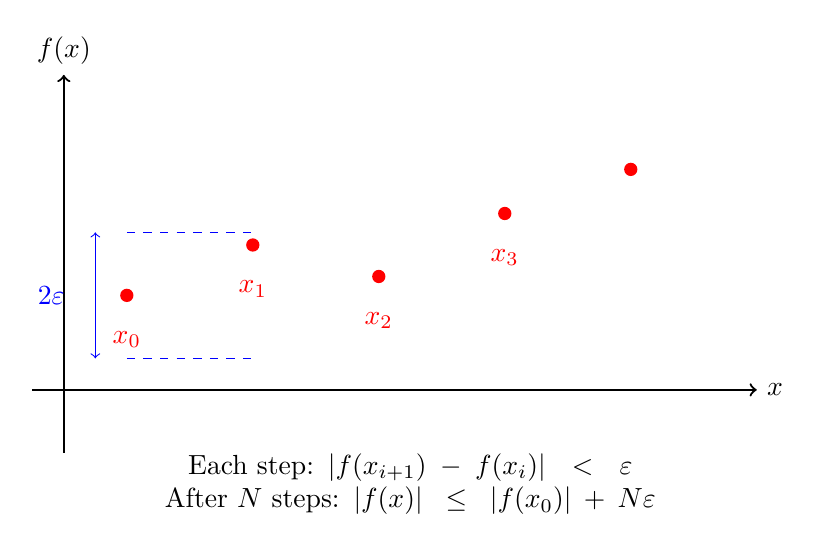
\begin{tikzpicture}[scale=0.8]
    \draw[thick, ->] (-0.5, 0) -- (11, 0) node[right] {$x$};
    \draw[thick, ->] (0, -1) -- (0, 5) node[above] {$f(x)$};

    % Chain of points
    \fill[red] (1, 1.5) circle (3pt);
    \fill[red] (3, 2.3) circle (3pt);
    \fill[red] (5, 1.8) circle (3pt);
    \fill[red] (7, 2.8) circle (3pt);
    \fill[red] (9, 3.5) circle (3pt);

    % Epsilon bands
    \draw[blue, dashed] (1, 0.5) -- (3, 0.5);
    \draw[blue, dashed] (1, 2.5) -- (3, 2.5);
    \draw[<->, blue] (0.5, 0.5) -- (0.5, 2.5);
    \node[blue] at (-0.2, 1.5) {$2\eps$};

    % Labels
    \node[red] at (1, 0.8) {$x_0$};
    \node[red] at (3, 1.6) {$x_1$};
    \node[red] at (5, 1.1) {$x_2$};
    \node[red] at (7, 2.1) {$x_3$};

    \node[text width=9cm, align=center] at (5.5, -1.5) {
        Each step: $|f(x_{i+1}) - f(x_i)| < \eps$\\
        After $N$ steps: $|f(x)| \leq |f(x_0)| + N\eps$
    };
\end{tikzpicture}
\end{center}

\textbf{More precisely:} For any $x \in E$, pick a reference point $x_0 \in E$. Walk from $x_0$ to $x$ in steps of at most $\delta$. You need at most $N = \lceil(b - a)/\delta\rceil$ steps. Each step changes $f$ by at most $\eps$, so:
\[
|f(x)| \leq |f(x_0)| + N \cdot \eps
\]
This bound is \textbf{finite} and works for all $x \in E$.

\section{Counterexample: Boundedness of $E$ is Needed}

\begin{center}
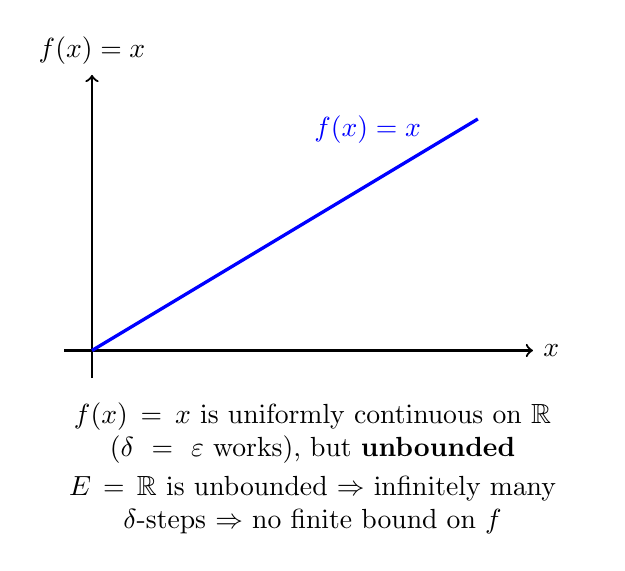
\begin{tikzpicture}[scale=0.7]
    \draw[thick, ->] (-0.5, 0) -- (8, 0) node[right] {$x$};
    \draw[thick, ->] (0, -0.5) -- (0, 5) node[above] {$f(x) = x$};

    \draw[blue, very thick, domain=0:7, samples=2] plot (\x, {0.6*\x});

    \node[blue] at (5, 4) {$f(x) = x$};
    \node[text width=7cm, align=center] at (4, -1.5) {$f(x) = x$ is uniformly continuous on $\R$\\($\delta = \eps$ works), but \textbf{unbounded}};
    \node[text width=7cm, align=center] at (4, -2.8) {$E = \R$ is unbounded $\Rightarrow$ infinitely many\\$\delta$-steps $\Rightarrow$ no finite bound on $f$};
\end{tikzpicture}
\end{center}

\section{Summary}

\begin{center}
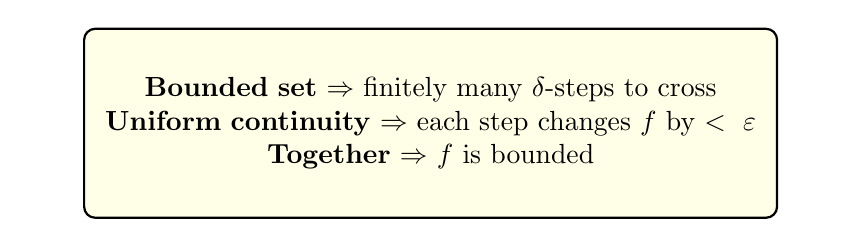
\begin{tikzpicture}[scale=0.8]
    \draw[thick, rounded corners, fill=yellow!10] (-5.5, -1.5) rectangle (5.5, 1.5);
    \node[text width=10cm, align=center] at (0, 0) {
        \textbf{Bounded set} $\Rightarrow$ finitely many $\delta$-steps to cross\\
        \textbf{Uniform continuity} $\Rightarrow$ each step changes $f$ by $< \eps$\\
        \textbf{Together} $\Rightarrow$ $f$ is bounded
    };
\end{tikzpicture}
\end{center}

\end{document}
